\documentclass[11pt]{amsart}

\usepackage{amsmath,amssymb,amsthm,mathtools}
\usepackage[margin=1.1in]{geometry}
\usepackage{enumitem}
\usepackage{tikz}
\usepackage[colorlinks=true,linkcolor=blue,citecolor=blue,urlcolor=blue]{hyperref}

\newtheorem{theorem}{Theorem}[section]
\newtheorem{proposition}[theorem]{Proposition}
\newtheorem{lemma}[theorem]{Lemma}
\newtheorem{corollary}[theorem]{Corollary}
\theoremstyle{definition}
\newtheorem{definition}[theorem]{Definition}
\newtheorem{example}[theorem]{Example}
\theoremstyle{remark}
\newtheorem{remark}[theorem]{Remark}
\numberwithin{equation}{section}

\newcommand{\C}{\mathbb{C}}
\newcommand{\Z}{\mathbb{Z}}
\newcommand{\R}{\mathbb{R}}
\newcommand{\F}{\mathbb{F}}
\newcommand{\cM}{\mathcal{M}}
\newcommand{\cH}{\mathcal{H}}
\newcommand{\cX}{\mathcal{X}}
\newcommand{\Afr}{\mathcal{A}^{\mathrm{fr}}}
\newcommand{\Aun}{\mathcal{A}^{0}}
\newcommand{\Om}{\Omega_m}
\newcommand{\norm}[1]{\lVert #1\rVert}
\newcommand{\gbin}[2]{\begin{bmatrix} #1 \\ #2 \end{bmatrix}_q}
\newcommand{\Em}{E_m}
\newcommand{\Lp}{(E_m)^{\lambda_S}_{+}}
\DeclareMathOperator{\Hilb}{Hilb}
\DeclareMathOperator{\Stab}{Stab}
\DeclareMathOperator{\id}{id}
\DeclareMathOperator{\wt}{wt}

\begin{document}

\title[Multipartition spaces, Kirwan perfection and Hausel's formula]{Multipartition spaces, Kirwan's
equivariant perfection,\\ and Hausel's formula}
\date{October 2026}

\begin{abstract}
These notes give a self-contained account of the geometric part of Section~6 of \cite{Hik}. For a
quiver with a loop at every vertex and a multipartition $m$, we define the multipartition quiver
$\Gamma_m$, the multipartition space $E_m$ and its open subset $U_m$, the torus $T_m$, the toric
hyperK\"ahler variety $Y_m$, and the action of the group $W_m$. We then prove
\cite[Proposition~6.2]{Hik} as an instance of Kirwan's equivariant perfection argument: the
decomposition of $E_m$ by the set of unreachable slots is exactly Hesselink's stratification for the
determinant character, in the terminology of Hoskins \cite{Hos}. Finally we recall Hausel's formula and
explain, following \cite[Corollary~6.3]{Hik}, how Proposition~6.2 computes the ratio of its two sums.

This note was written by Claude Opus 5.5 (Anthropic) at the request of Hiraku Nakajima, based on a
discussion with him in October 2026. A record of the discussion is available on request.
\end{abstract}

\maketitle

\setcounter{tocdepth}{1}
\tableofcontents

\section*{Conventions}

Equation, proposition and corollary numbers of the form (6.1), Proposition~6.2, Corollary~6.3 refer to
\cite{Hik}. All other numbers are cross-references within this note and are hyperlinks to the
corresponding statement or equation.

Cohomology has complex coefficients, and equivariant cohomology is Borel equivariant cohomology. All
graded vector spaces below are concentrated in even degrees, finite-dimensional in each degree and
bounded below; for such a space we put
\[
  \Hilb(M;q)=\sum_{d}\dim M^{2d}\,q^{d}.
\]
Thus $q$ records \emph{half} the cohomological degree. If $X$ has no odd cohomology, its Poincar\'e
polynomial is $P_X(q)=\Hilb(H^*(X);q)$, and $P_\emptyset=0$.

For geometric invariant theory of a linear action on an affine space with respect to a character we
follow the terminology and notation of Hoskins \cite[\S2]{Hos}. In \S\ref{subsec:stab} and
Section~\ref{sec:kirwan}, $\lambda$ denotes a one-parameter subgroup; elsewhere $\lambda=(\lambda^i)$
denotes a tuple of partitions.

In \cite{Hik} the polynomials $h_m$ defined below bound the graded pieces of a filtration of the
Coulomb-side ring $B_0$ \cite[Proposition~5.2]{Hik}; Hausel's formula shows that the bound is sharp
\cite[Proposition~6.4, Corollary~6.6]{Hik}. We do not revisit that part of the argument.

\section{Multipartition spaces}\label{sec:defs}

\subsection{The quiver}\label{subsec:quiver}
Let $Q=(Q_0,Q_1)$ be a finite quiver with at least one loop at every vertex. For an arrow $a\in Q_1$ we
write $t(a)$ and $h(a)$ for its tail and head. Fix one loop $\ell_i$ at each vertex $i$, and let $Q'$ be
the quiver obtained from $Q$ by deleting the chosen loops. Put
\begin{equation}\label{eq:cij}
  n_{ij}=\#\{a\in Q'_1: t(a)=i,\ h(a)=j\},\qquad c_{ij}=n_{ij}+n_{ji}.
\end{equation}
The matrix $(c_{ij})$ is symmetric with nonnegative integer entries, and $c_{ii}=2n_{ii}$ is even.
Fix a framing vector $w\in\Z_{\ge 0}^{Q_0}$. For $v\in\Z_{\ge0}^{Q_0}$ put
\begin{equation}\label{eq:Cv}
  C(v)=\tfrac12\sum_{i,j}c_{ij}v_iv_j=\sum_{a\in Q'_1}v_{t(a)}v_{h(a)}.
\end{equation}

\subsection{Multipartitions}\label{subsec:multipartitions}

\begin{definition}\label{def:multipartition}
A \emph{multipartition} is a family $m=(m_{i,s})_{i\in Q_0,\,s\ge1}$ of nonnegative integers, only
finitely many of which are nonzero. Its \emph{dimension vector} $\norm{m}\in\Z_{\ge0}^{Q_0}$ is
$\norm{m}_i=\sum_{s}s\,m_{i,s}$, and $m$ is called a multipartition of $v$ if $\norm{m}=v$. Let $\cM$ be
the set of all multipartitions (of all dimension vectors) and $\cM(v)\subset\cM$ the finite subset of
multipartitions of $v$. The empty multipartition $\emptyset$ is the unique multipartition of $0$.
\end{definition}

Equivalently, $m$ is a $Q_0$-tuple $\lambda=(\lambda^i)_{i\in Q_0}$ of partitions, where $m_{i,s}$ is the
number of parts of $\lambda^i$ equal to $s$; we write $m=m(\lambda)$ and use both descriptions.

\begin{definition}\label{def:notation}
For $k,m\in\cM$ put
\begin{gather}
  l_i(m)=\textstyle\sum_s m_{i,s}\ \text{(the number of parts at $i$)},\qquad
  l(m)=(l_i(m))_i,\qquad |l(m)|=\textstyle\sum_i l_i(m),\label{eq:l}\\
  w(m)=w\cdot l(m)=\textstyle\sum_i w_i\,l_i(m),\qquad
  (q)_m=\prod_{i,s}\prod_{j=1}^{m_{i,s}}(1-q^j),\label{eq:qm}\\
  b(k,m)=\sum_{i,j\in Q_0}\sum_{s,t\ge1}c_{ij}\min(s,t)\,k_{i,s}\,m_{j,t},\qquad D_m=\tfrac12\,b(m,m).
  \label{eq:b}
\end{gather}
\end{definition}

The form $b$ is bilinear and symmetric. For partitions put $\langle\mu,\nu\rangle=\sum_{a,b}\min(\mu_a,\nu_b)$;
then
\begin{equation}\label{eq:Dm}
  D_{m(\lambda)}=\tfrac12\sum_{i,j}c_{ij}\langle\lambda^i,\lambda^j\rangle
  =\sum_{a\in Q'_1}\langle\lambda^{t(a)},\lambda^{h(a)}\rangle\in\Z_{\ge0}.
\end{equation}
Multipartitions are added entrywise, and $\norm{k+m}=\norm{k}+\norm{m}$. We write $k\le m$ if
$k_{i,s}\le m_{i,s}$ for all $(i,s)$; then $m-k\in\cM$. Bilinearity gives
\begin{equation}\label{eq:additivity}
  D_{k+m'}=D_k+D_{m'}+b(k,m'),\qquad w(k+m')=w(k)+w(m').
\end{equation}

\subsection{The multipartition quiver and slots}\label{subsec:Gamma}

\begin{definition}\label{def:Gamma}
Let $m\in\cM$ and put $\Om=\{(i,s,\alpha): i\in Q_0,\ s\ge1,\ 1\le\alpha\le m_{i,s}\}$. The
\emph{multipartition quiver} $\Gamma_m$ has vertex set $\Om\sqcup\{\infty\}$. The vertex $\infty$ is the
\emph{framing vertex}; the other vertices, i.e.\ the elements of $\Om$, are called \emph{slots}. A slot
$d=(i,s,\alpha)$ has \emph{color} $i(d)=i$, \emph{size} $s(d)=s$ and \emph{type} $(i,s)$. For distinct
slots $d\neq e$ put
\begin{equation}\label{eq:bde}
  b_{de}=c_{i(d)i(e)}\min(s(d),s(e))=b_{ed}.
\end{equation}
The arrows of $\Gamma_m$ are:
\begin{itemize}[leftmargin=2em]
\item for every ordered pair $(d,e)$ of distinct slots, $b_{de}$ arrows $d\to e$, labeled
$(d\to e,p)$ with $1\le p\le b_{de}$;
\item for every slot $d$, $w_{i(d)}$ \emph{framing arrows} $\infty\to d$, labeled $(\infty\to d,p)$ with
$1\le p\le w_{i(d)}$.
\end{itemize}
\end{definition}

There are $m_{i,s}$ slots of type $(i,s)$ and $|l(m)|$ slots in all; the sizes of the slots of color $i$
are the parts of $\lambda^i$. By \eqref{eq:bde}, the full subquiver on the slots is \emph{symmetric}: it
has as many arrows $d\to e$ as $e\to d$. There are no arrows into $\infty$ and no loops.

The group
\begin{equation}\label{eq:Wm}
  W_m=\prod_{i,s}\mathfrak S_{m_{i,s}}
\end{equation}
acts on $\Om$ by $\sigma(i,s,\alpha)=(i,s,\sigma_{i,s}(\alpha))$. Thus $W_m$ is the group of permutations
of the slots preserving types, and $b_{\sigma d,\sigma e}=b_{de}$.

For $S\subseteq\Om$ its \emph{type} is the multipartition $\kappa(S)=k\le m$ with
$k_{i,s}=\#\{d\in S\text{ of type }(i,s)\}$; the complement $\Om\setminus S$ has type $m-k$. Two subsets
lie in the same $W_m$-orbit if and only if they have the same type, and the stabilizer of $S$ is
$W_k\times W_{m-k}$. We identify
\begin{equation}\label{eq:ident}
  \Om\setminus S\ \cong\ \Omega_{m-k}
\end{equation}
by the type-preserving, order-preserving relabeling of the index $\alpha$; this identification preserves
the numbers $b_{de}$. By definition of $b$ in \eqref{eq:b},
\begin{equation}\label{eq:bcross}
  b(\kappa(S),\,m-\kappa(S))=\sum_{d\in S}\ \sum_{e\in\Om\setminus S} b_{de},
  \qquad
  D_m=\sum_{\{d,e\},\,d\neq e} b_{de}+\sum_{d\in\Om} n_{i(d)i(d)}\,s(d).
\end{equation}
In the second formula the sum is over unordered pairs; the last term comes from the pairs $d=e$ in
$\frac12 b(m,m)$ and vanishes when $Q'$ has no loops.

\subsection{The multipartition space}\label{subsec:Em}

\begin{definition}\label{def:Em}
The \emph{multipartition space} $E_m$ is the space of representations of the multipartition quiver
$\Gamma_m$ (Definition~\ref{def:Gamma}) with a one-dimensional space $\C$ at every vertex:
\[
  E_m=E_m^{\mathrm{int}}\oplus F_m,\qquad
  E_m^{\mathrm{int}}=\bigoplus_{d\neq e}\C^{b_{de}},\qquad
  F_m=\bigoplus_{d\in\Om}\C^{w_{i(d)}}.
\]
We write a point as $B=(B',a)$, where $B'=(B^{(p)}_{d\to e})\in E_m^{\mathrm{int}}$ consists of the
components $B^{(p)}_{d\to e}$, $1\le p\le b_{de}$, for the arrows between slots, and
$a=(a^{(p)}_d)\in F_m$ consists of the components $a^{(p)}_d$, $1\le p\le w_{i(d)}$, for the framing
arrows.
\end{definition}

Thus $\dim E_m=2\sum_{\{d,e\}}b_{de}+w(m)$, and $E_\emptyset$ is a point.

\subsection{The torus and the cut ideal}\label{subsec:torus}
The torus $T_m=(\C^\times)^{\Om}$ acts on $E_m$ by change of basis at the slots, trivially at $\infty$:
\begin{equation}\label{eq:Taction}
  t\cdot(B',a):\quad B^{(p)}_{d\to e}\mapsto t_e\,t_d^{-1}\,B^{(p)}_{d\to e},\qquad
  a^{(p)}_d\mapsto t_d\,a^{(p)}_d .
\end{equation}
Let $x_d\in H^2_{T_m}(\mathrm{pt})$ be the first Chern class of the character $t\mapsto t_d$, so that
\[
  P_m:=H^*_{T_m}(\mathrm{pt})=\C[x_d:d\in\Om],\qquad \deg x_d=2 .
\]
By \eqref{eq:Taction} the weights of $E_m$ are
\begin{equation}\label{eq:weights}
  x_e-x_d\ \text{ on each coordinate } B^{(p)}_{d\to e},\qquad x_d\ \text{ on each coordinate } a^{(p)}_d .
\end{equation}
Since $E_m$ is contractible, $H^*_{T_m}(E_m)=P_m$.

\begin{definition}\label{def:cut}
For a nonempty subset $S\subseteq\Om$, the \emph{cut polynomial} \cite[(5.3)]{Hik} is
\[
  q_S=\prod_{d\in S}x_d^{\,w_{i(d)}}\prod_{d\in S,\ e\notin S}(x_d-x_e)^{b_{de}}\in P_m .
\]
The \emph{cut ideal} $J_m\subseteq P_m$ is the ideal generated by all $q_S$, and
\[
  h_m(q)=\Hilb\big((P_m/J_m)^{W_m};q\big),
\]
where $W_m$ acts on $P_m/J_m$ as in \S\ref{subsec:Wm}.
\end{definition}

We keep the notation of \cite{Hik}; $q_S$ has nothing to do with the variable $q$. By
\cite[Lemma~6.1]{Hik}, $P_m/J_m$ is finite-dimensional, so $h_m$ is a polynomial. This also follows from
Remark~\ref{rem:Ym}\ref{it:HS}: there $P_m/J_m$ is identified with the cohomology of the toric
hyperK\"ahler variety $Y_m$, whose Betti numbers $b_{2k}$ are the $h$-numbers $h_k$, $0\le k\le g_m$, of a
matroid of rank $g_m$ \cite[Corollaries~4.6 and~6.6]{HS}, where $g_m$ is as in
Remark~\ref{rem:Ym}\ref{it:dim}. Hence $P_m/J_m$ vanishes in degrees above $2g_m$, and $h_m$ has degree at
most $g_m$. For $m=\emptyset$ we have $P_\emptyset=\C$, $J_\emptyset=0$ and $h_\emptyset=1$.

\subsection{The action of \texorpdfstring{$W_m$}{W\_m}}\label{subsec:Wm}
The arrow labels in Definition~\ref{def:Gamma} depend only on the types of the endpoints, so the group
$W_m$ of \eqref{eq:Wm} acts on $\Gamma_m$, and hence on $E_m$ and on $T_m$:
\[
  (\sigma B)^{(p)}_{\sigma d\to\sigma e}=B^{(p)}_{d\to e},\qquad (\sigma a)^{(p)}_{\sigma d}=a^{(p)}_d,\qquad
  (\sigma t)_{\sigma d}=t_d .
\]
These satisfy $\sigma(t\cdot B)=(\sigma t)\cdot(\sigma B)$, so the semidirect product $T_m\rtimes W_m$
acts on $E_m$. (It is the normalizer of the maximal torus in $\prod_{i,s}GL_{m_{i,s}}$.) If
$\cX\subseteq E_m$ is stable under $T_m\rtimes W_m$, each $\sigma$ gives an equivariant automorphism of
$(\cX,T_m)$; letting $\sigma$ act by $(\sigma^{-1})^*$ defines a left action of $W_m$ on $H^*_{T_m}(\cX)$
by graded algebra automorphisms. On $H^*_{T_m}(\mathrm{pt})=P_m$ it is $\sigma\cdot x_d=x_{\sigma d}$. We
record three facts.
\begin{enumerate}[label=(\alph*),leftmargin=2em]
\item\label{fact:inv} Since $W_m$ is finite and coefficients are complex, taking $W_m$-invariants is
exact, and
\[
  H^*_{T_m\rtimes W_m}(\cX)=H^*_{T_m}(\cX)^{W_m}.
\]
\item\label{fact:J} $\sigma\cdot q_S=q_{\sigma S}$, hence $J_m$ is $W_m$-stable and $W_m$ acts on
$P_m/J_m$.
\item\label{fact:qm} $P_m^{W_m}$ is the tensor product over $(i,s)$ of rings of symmetric polynomials in
$m_{i,s}$ variables, so $\Hilb(P_m^{W_m};q)=1/(q)_m$, with $(q)_m$ as in \eqref{eq:qm}.
\end{enumerate}

\subsection{Stability for the torus action}\label{subsec:stab}
We use the notation of \cite[\S2]{Hos}, specialized to the torus $T_m$ acting on $E_m$. Characters and
one-parameter subgroups (1-PSs) of $T_m$ are identified with vectors in $\Z^{\Om}$: a character $\chi$
is $t\mapsto\prod_dt_d^{\chi_d}$, a 1-PS $\lambda$ is $\tau\mapsto(\tau^{\lambda_d})_d$, and the pairing
is $(\chi,\lambda)=\sum_d\chi_d\lambda_d$. We write characters additively, so $x_d$ is the character
$t\mapsto t_d$, and we use the standard norm $\norm{\lambda}^2=\sum_d\lambda_d^2$, which is invariant
under $W_m$ and satisfies \cite[Assumption~2.9]{Hos}. For $A\subseteq\Om$ let
$1_A\in\Z^{\Om}$ have entries $1$ on $A$ and $0$ elsewhere. Throughout, the character is
\begin{equation}\label{eq:rho}
  \rho=\det=1_{\Om}:\ T_m\to\C^\times,\qquad t\mapsto\prod_dt_d .
\end{equation}
In King's notation for the quiver $\Gamma_m$, this is the stability parameter which is $1$ at every
slot \cite[\S5.1]{Hos}.

\begin{definition}[{\cite[Definition~2.1]{Hos}}]\label{def:stab}
A point $B\in E_m$ is \emph{$\rho$-semistable} if there are $n>0$ and $f\in\C[E_m]$ with
$f(t\cdot B'')=\rho(t)^nf(B'')$ for all $t\in T_m$, $B''\in E_m$, and $f(B)\neq0$. It is
\emph{$\rho$-stable} if moreover its stabilizer is finite and $T_m$ acts on $\{f\neq0\}$ with closed
orbits, for some such $f$. Otherwise $B$ is \emph{$\rho$-unstable}. We write
$E_m^{\rho\text{-}s}\subseteq E_m^{\rho\text{-}ss}$ for the open subsets of $\rho$-stable and
$\rho$-semistable points, and $E_m/\!/_\rho T_m$ for the GIT quotient.
\end{definition}

For $B\in E_m$ let $\wt(B)$ be the set of weights $\chi$ in \eqref{eq:weights} such that the component
of $B$ in the $\chi$-weight space is nonzero. Following \cite[(4)]{Hos}, the \emph{cone of allowable
1-PSs} of $B$ is
\begin{equation}\label{eq:CB}
  C_B=\bigcap_{\chi\in\wt(B)}H_\chi\subseteq\R^{\Om},\qquad
  H_\chi=\{\lambda:(\chi,\lambda)\ge0\}.
\end{equation}
A 1-PS $\lambda$ lies in $C_B$ if and only if $\lim_{\tau\to0}\lambda(\tau)\cdot B$ exists. Put
$H_\rho=\{\lambda:(\rho,\lambda)\ge0\}$ and $H_\rho^{\circ}=\{\lambda:(\rho,\lambda)>0\}$.

\begin{proposition}[Hilbert--Mumford criterion {\cite[\S2.1]{Hos}}]\label{prop:HM}
Let $B\in E_m$ and recall $C_B$ from \eqref{eq:CB}. Then $B$ is $\rho$-semistable if and only if
$C_B\subseteq H_\rho$, and $\rho$-stable if and only if $C_B\setminus\{0\}\subseteq H_\rho^{\circ}$.
\end{proposition}

\subsection{Reachability and \texorpdfstring{$U_m$}{U\_m}}\label{subsec:Um}

\begin{definition}\label{def:reach}
Let $B=(B',a)\in E_m$ (Definition~\ref{def:Em}). A slot $d$ is \emph{reachable} in $B$ if there are slots
$d_1,\dots,d_r=d$ ($r\ge1$) and labels such that $a^{(p_0)}_{d_1}\neq0$ and
$B^{(p_j)}_{d_j\to d_{j+1}}\neq0$ for $1\le j<r$. Let $R(B)$ be the set of reachable slots and
$S(B)=\Om\setminus R(B)$ the set of unreachable ones. Put
\[
  U_m=\{B\in E_m: R(B)=\Om\}.
\]
For $S\subseteq\Om$ let $\lambda_S=-1_S$ be the 1-PS with $\lambda_S(\tau)_d=\tau^{-1}$ for $d\in S$ and
$1$ otherwise; $\lambda_\emptyset$ is the trivial 1-PS.
\end{definition}

``$d$ is reachable'' is a finite union of non-vanishing conditions, so $U_m$ is open; it is stable under
$T_m\rtimes W_m$ (\S\ref{subsec:Wm}).

\begin{lemma}\label{lem:key}
Let $B\in E_m$. Recall the sets $R(B)$, $S(B)$ and the 1-PS $\lambda_S$ of
Definition~\ref{def:reach}, and the cone $C_B$ of \eqref{eq:CB}.
\begin{enumerate}[label=(\arabic*),leftmargin=2em]
\item\label{key:pos} Every $\lambda\in C_B$ satisfies $\lambda_d\ge0$ for all $d\in R(B)$.
\item\label{key:lambda} $\lambda_{S(B)}\in C_B$, and $(\rho,\lambda_{S(B)})=-|S(B)|$.
\end{enumerate}
\end{lemma}

\begin{proof}
\ref{key:pos} Take a path $d_1,\dots,d_r=d$ as in Definition~\ref{def:reach}. By \eqref{eq:weights},
$x_{d_1}\in\wt(B)$ and $x_{d_{j+1}}-x_{d_j}\in\wt(B)$, so $\lambda_{d_1}\ge0$ and
$\lambda_{d_{j+1}}\ge\lambda_{d_j}$; hence $\lambda_d\ge0$.

\ref{key:lambda} Put $S=S(B)$ and $R=R(B)$. A nonzero framing coordinate $a_d$ with $d\in S$, or a nonzero
coordinate $B_{e\to d}$ with $e\in R$, $d\in S$, would make $d$ reachable; so these vanish. The remaining
weights in $\wt(B)$ are $x_d$ with $d\in R$, $x_e-x_d$ with $d,e$ both in $R$ or both in $S$, and
$x_e-x_d$ with $d\in S$, $e\in R$. Their pairings with $\lambda_S=-1_S$ are $0$, $0$ and $1$, all
$\ge0$. Finally $(\rho,\lambda_S)=-|S|$ by \eqref{eq:rho}.
\end{proof}

\begin{lemma}\label{lem:Um}
Let $B\in E_m$, and recall $\rho$-(semi)stability from Definition~\ref{def:stab}.
\begin{enumerate}[label=(\arabic*),leftmargin=2em]
\item\label{Um:cyclic} The smallest subrepresentation of $B$ containing the space at $\infty$ is
supported on $\{\infty\}\cup R(B)$. Hence $B\in U_m$ if and only if $B$ is cyclic, i.e.\ generated by
the space at $\infty$.
\item\label{Um:ss} $U_m=E_m^{\rho\text{-}ss}=E_m^{\rho\text{-}s}$.
\item\label{Um:free} $T_m$ acts freely on $U_m$. The quotient $U_m/T_m=E_m/\!/_\rho T_m$ is a smooth
quasi-projective toric variety of dimension $\dim E_m-|l(m)|$ (if nonempty), and
\[
  H^*_{T_m}(U_m)=H^*(U_m/T_m),\qquad H^*_{T_m}(U_m)^{W_m}=H^*\big((U_m/T_m)/W_m\big).
\]
\end{enumerate}
\end{lemma}

\begin{proof}
\ref{Um:cyclic} All vertex spaces are one-dimensional, so a subrepresentation is a subset of vertices
closed under nonzero arrows. The smallest one containing $\infty$ is $\{\infty\}\cup R(B)$.

\ref{Um:ss} If $B\in U_m$, then every $0\neq\lambda\in C_B$ has $\lambda_d\ge0$ for all $d$ by
Lemma~\ref{lem:key}\ref{key:pos}, hence $(\rho,\lambda)=\sum_d\lambda_d>0$. By
Proposition~\ref{prop:HM}, $B$ is $\rho$-stable. If $S(B)\neq\emptyset$, then
Lemma~\ref{lem:key}\ref{key:lambda} gives $\lambda_{S(B)}\in C_B$ with $(\rho,\lambda_{S(B)})<0$, so
$C_B\not\subseteq H_\rho$ and $B$ is $\rho$-unstable.

\ref{Um:free} If $t\cdot B=B$, then $t_d=1$ whenever $a_d\neq0$, and $t_e=t_d$ whenever
$B_{d\to e}\neq0$; following paths from $\infty$ gives $t=1$. By \ref{Um:ss} and \cite[Theorem~2.2]{Hos},
$U_m\to E_m/\!/_\rho T_m$ is a geometric quotient, smooth because the action is free. The torus
$(\C^\times)^{\dim E_m}$ scaling all coordinates commutes with $T_m$ and preserves $U_m$, since
reachability only depends on which coordinates are nonzero. If $U_m\neq\emptyset$, it contains the open
orbit where all coordinates are nonzero, so $U_m/T_m$ is toric. The last assertions hold because the
action is free and $W_m$ is finite.
\end{proof}

\subsection{The toric hyperK\"ahler variety \texorpdfstring{$Y_m$}{Y\_m}}\label{subsec:Ym}
Choose an \emph{orientation} $o$: for every unordered pair $\{d,e\}$ of distinct slots and every
$1\le p\le b_{de}$, declare one of $(d\to e,p)$, $(e\to d,p)$ to be \emph{original}. Let $V^o_m$ be the
framed quiver with vertex set $\Om\sqcup\{\infty\}$, the original arrows and the framing arrows, and let
\[
  L^o_m=\bigoplus_{\text{original arrows}}\C\ \oplus\ F_m
\]
be its representation space with dimension vector $1$. The coordinate of the reverse $\bar\gamma$ of an
original arrow $\gamma$ has the opposite weight, so it is naturally dual to the coordinate $B_\gamma$.
Hence
\[
  T^*L^o_m=L^o_m\oplus(L^o_m)^\vee=E_m\oplus F_m^\vee,\qquad
  F_m^\vee=\bigoplus_d\big(\C^{w_{i(d)}}\big)^\vee,
\]
where the coordinates $b_d=(b^{(p)}_d)_p$ of $F_m^\vee$ are dual framing arrows $d\to\infty$, of weight
$-x_d$. Following the recent literature we write $b$ for the dual framing; it should not be confused with
the integers $b_{de}$ of \eqref{eq:bde} or the bilinear form $b(k,m)$ of \eqref{eq:b}. The
moment map $\mu:E_m\oplus F_m^\vee\to\operatorname{Lie}(T_m)^\vee=\C^{\Om}$, defined by
$\langle\mu(s,p),\xi\rangle=\langle p,\xi\cdot s\rangle$ as in \cite{Hik}, is
\[
  \mu_d(B,b)=\sum_{\substack{\gamma\text{ original}\\ h(\gamma)=d}}B_\gamma B_{\bar\gamma}
       -\sum_{\substack{\gamma\text{ original}\\ t(\gamma)=d}}B_\gamma B_{\bar\gamma}
       +\langle b_d,a_d\rangle ,\qquad \langle b_d,a_d\rangle=\sum_pb^{(p)}_da^{(p)}_d .
\]

\begin{definition}\label{def:Ym}
$Y_m=\{(B,b)\in U_m\times F_m^\vee:\ \mu(B,b)=0\}/T_m$, where $B=(B',a)\in U_m$ and $b\in F_m^\vee$.
\end{definition}

\begin{remark}\label{rem:Ym}
\begin{enumerate}[label=(\roman*),leftmargin=2em]
\item\label{it:qv} $Y_m$ is the quiver variety \cite{Nak} of $V^o_m$ with dimension vector $(1,\dots,1)$
and framing $w$, in its holomorphic description at determinant stability (cf.\
\cite[Theorem~3.2, Proposition~3.5]{Nak}). The multipartition quiver has no edge loops, so this is within
the setting of \cite{Nak}. Indeed, by the argument of Lemma~\ref{lem:Um}\ref{Um:cyclic}, cyclicity in the
doubled quiver means reachability using the framing arrows $\infty\to d$ and the arrows between slots in
both directions; that is exactly the condition $B\in U_m$, and the dual framing $b$ plays no role.
\item\label{it:dim} $T_m$ acts freely on $U_m\times F_m^\vee$ (Lemma~\ref{lem:Um}\ref{Um:free}), so
$\mu$ is a submersion there and $Y_m$ is smooth of dimension
\[
  \dim Y_m=2g_m,\qquad g_m=\sum_{\{d,e\}}b_{de}+w(m)-|l(m)|.
\]
Here $g_m$ is the number of edges minus the number of slots of the underlying graph of $\Gamma_m$, i.e.\
its first Betti number when that graph is connected.
\item\label{it:orient} Changing the orientation changes the sign of some terms of $\mu$. Changing the
sign of the corresponding reverse coordinates is a $T_m$-equivariant isomorphism, so $Y_m$ does not depend
on $o$ up to isomorphism. Composing with such sign changes, $W_m$ acts on $Y_m$.
\item\label{it:HS} \emph{Relation with Hausel--Sturmfels \cite{HS}.} Let $A$ be the integer matrix with
$|l(m)|$ rows whose columns are the $T_m$-weights \eqref{eq:weights} of the coordinates of $L^o_m$, one
column for each original arrow and each framing arrow. This is the boundary map \cite[(40)]{HS} of the
quiver $V^o_m$, with $v_0=\infty$; it is unimodular \cite[Lemma~8.1]{HS}, and $T_m$ plays the role of the
torus $\mathbb T^d_\C$ of \cite{HS}. The character $\rho=\det$ of \eqref{eq:rho} is the vector
$\theta=(1,\dots,1)$ of \cite{HS}. A hyperplane spanned by columns of $A$ is spanned by the arrows of a
forest with two components; if $S\subseteq\Om$ is the component not containing $\infty$, the hyperplane
is $\{y:\sum_{d\in S}y_d=0\}$. Since $\sum_{d\in S}\theta_d=|S|\neq0$, $\theta$ is generic in the sense of
\cite[\S4]{HS}. In this notation:
\begin{itemize}[leftmargin=1.5em]
\item The coordinates $z_i,w_i$ of \cite[\S4]{HS} are the coordinates of $L^o_m$ and their duals, so the
Lawrence toric variety of \cite[Definition~4.1, Theorem~1.1(2)]{HS} is the GIT quotient of
$T^*L^o_m=E_m\oplus F_m^\vee$ without the moment map equation:
\[
  X^{\mathrm{Law}}_m:=X(A^\pm,\theta)=(E_m\oplus F_m^\vee)/\!/_\rho\,T_m .
\]
\item $Y_m$ is the toric quiver variety $Y(V^o_m,\theta)=Y(A,\theta)$ of \cite[\S8]{HS}: the subvariety of
$X^{\mathrm{Law}}_m$ cut out by the components of the complex moment map \cite[(29),
Definition~6.1]{HS}, biholomorphic to the hyperK\"ahler quotient \cite[Theorem~6.3]{HS}. (In
\cite[\S6]{HS} the Gale dual matrix is assumed to have no zero row, i.e.\ the underlying graph has no
bridge, so that the ideal (29) is prime; in general we take Definition~\ref{def:Ym} as the definition.)
\item $X^{\mathrm{Law}}_m$ is a vector bundle over the toric manifold $U_m/T_m$, whose fiber consists of
the linear maps \emph{to} the framing vector spaces. Indeed, the coordinates $b_d$ of $F_m^\vee$ are arrows
$d\to\infty$, which do not help to reach slots from $\infty$; so Lemma~\ref{lem:key}\ref{key:pos} still
holds for the cone of allowable 1-PSs of $(B,b)$. Their weights $-x_d$ pair with $\lambda_{S(B)}$ to
$0$ or $1$, so Lemma~\ref{lem:key}\ref{key:lambda} also holds. The proof of
Lemma~\ref{lem:Um}\ref{Um:ss} then shows that the semistable locus is $U_m\times F_m^\vee$, on which $T_m$
acts freely. Therefore
\[
  X^{\mathrm{Law}}_m=U_m\times^{T_m}F_m^\vee=\bigoplus_{d\in\Om}\operatorname{Hom}\big(\mathcal L_d,\,\C^{w_{i(d)}}\big),
\]
where $\mathcal L_d$ is the line bundle on $U_m/T_m$ associated with the character $t\mapsto t_d$ (the
tautological line at the slot $d$), and $\C^{w_{i(d)}}$ is a trivial bundle. The zero section is
$U_m/T_m$, and $Y_m\subset X^{\mathrm{Law}}_m$ is the closed subvariety $\mu=0$. For a single slot with $w$
framing arrows this is the example in \cite[\S1]{HS}: a rank $w$ bundle over $\mathbb P^{w-1}$ containing
$Y_m=T^*\mathbb P^{w-1}$.
\item By \cite[Theorem~1.1]{HS} and the remark after its proof, $Y_m$, $X^{\mathrm{Law}}_m$ and their
common core are deformation retracts of one another, and their cohomology (with $\Z$ coefficients, as $A$
is unimodular) is $\Z[x_1,\dots,x_N]/(\mathrm{Circ}(A)+M^*(A))$, where $N$ is the number of columns of $A$
and there is one variable for each column. By \cite[Theorem~8.3]{HS}, $M^*(A)$ is generated by the
monomials of the cuts of the underlying graph. In the presentation \cite[(37)]{HS}, which eliminates
$\mathrm{Circ}(A)$, each variable is replaced by the weight of its arrow, a linear form in the $x_d$; the
monomial of the cut separating $S$ from $(\Om\setminus S)\cup\{\infty\}$ then becomes $\pm q_S$
(Definition~\ref{def:cut}). Hence
\[
  H^*(Y_m)\cong H^*(X^{\mathrm{Law}}_m)\cong P_m/J_m ,
\]
and $J_m$ is the image of the cocircuit ideal; compare \cite[Section~5.1]{Hik}. Combined with the vector
bundle structure, this gives a second proof of Proposition~\ref{prop:62}\ref{62:a}, the map
$P_m\to H^*(U_m/T_m)$ sending $x_d$ to $c_1(\mathcal L_d)$. By \cite[Corollary~8.4]{HS}, the Euler
characteristic of $Y_m$ is the number of spanning trees of the underlying graph; for $m_b$ in
Example~\ref{ex:A2} it is $4$. (If some component of the graph misses $\infty$, then $U_m=\emptyset$ and
$J_m=P_m$, so all these spaces are empty.)
\end{itemize}
Apart from the alternative argument for the finite-dimensionality of $P_m/J_m$ in \S\ref{subsec:torus},
none of this is used in what follows.
\item\label{it:CBVdB} Applying Crawley-Boevey--Van den Bergh \cite{CBVdB} to $V^o_m$ with dimension
vector $(1,\dots,1)$, and using \ref{it:HS} and purity, the number $a_m(q)$ of absolutely indecomposable
representations of $V^o_m$ of this dimension over $\F_q$ is $a_m(q)=q^{-g_m}\#Y_m(\F_q)
=q^{g_m}\Hilb(P_m/J_m;q^{-1})$. By Kac, $a_m$ does not depend on $o$. This is also not used below.
\end{enumerate}
\end{remark}

\begin{example}\label{ex:A2}
Let $Q$ be the quiver $1\to2$ with a loop added at each vertex, so $Q'$ is $1\to 2$, $c_{12}=c_{21}=1$
and $c_{11}=c_{22}=0$ in \eqref{eq:cij}. Take $v=(2,1)$ and $w=(1,0)$. Then $C(v)=2$, and $\cM(v)$
consists of
\[
  m_a:\ \lambda^1=(2),\ \lambda^2=(1),\qquad m_b:\ \lambda^1=(1,1),\ \lambda^2=(1).
\]
For $m_b$ there are slots $d_1,d_2$ of type $(1,1)$ and $e$ of type $(2,1)$, with $b_{d_1e}=b_{d_2e}=1$
and $b_{d_1d_2}=c_{11}=0$; $W_{m_b}=\mathfrak S_2$ swaps $d_1,d_2$. The multipartition quiver is
\begin{center}
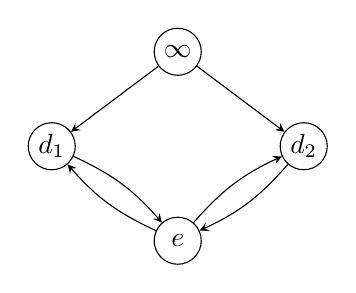
\begin{tikzpicture}[>=stealth, every node/.style={circle, draw, inner sep=1pt, minimum size=17pt}]
\node (inf) at (0,0) {$\infty$};
\node (d1) at (-1.6,-1.2) {$d_1$};
\node (d2) at (1.6,-1.2) {$d_2$};
\node (e) at (0,-2.4) {$e$};
\draw[->] (inf) -- (d1);
\draw[->] (inf) -- (d2);
\draw[->, bend left=12] (d1) to (e);
\draw[->, bend left=12] (e) to (d1);
\draw[->, bend left=12] (d2) to (e);
\draw[->, bend left=12] (e) to (d2);
\end{tikzpicture}
\end{center}
so $\dim E_{m_b}=6$ and $U_{m_b}/T_{m_b}$ is a smooth toric threefold. Its underlying graph is a
$4$-cycle, $g_{m_b}=1$, and $Y_{m_b}$ is the $A_3$-surface. Writing $a=x_{d_1}$, $b=x_{d_2}$, $c=x_e$,
the cut polynomials of Definition~\ref{def:cut} are
\[
  a(a-c),\ b(b-c),\ (c-a)(c-b),\ a(c-b),\ b(c-a),\ ab,\ ab(a-c)(b-c),
\]
for $S=\{d_1\},\{d_2\},\{e\},\{d_1,e\},\{d_2,e\},\{d_1,d_2,e\},\{d_1,d_2\}$ respectively. They generate
$J_{m_b}=(a,b,c)^2$. Hence $P_{m_b}/J_{m_b}$ has basis $1,a,b,c$, with Hilbert series $1+3q$, and
$h_{m_b}=1+2q$ (invariants $1$, $a+b$, $c$).

For $m_a$ there are slots $d$ of type $(1,2)$ and $e$ of type $(2,1)$, with $b_{de}=\min(2,1)=1$; the
multipartition quiver is $\infty\to d\rightleftarrows e$. Then $J_{m_a}=(x_d,x_e)$ and $h_{m_a}=1$.
\end{example}

\section{Proposition 6.2 via Kirwan's equivariant perfection}\label{sec:kirwan}

Recall the multipartition space $E_m$ (Definition~\ref{def:Em}) and its open subset $U_m$
(Definition~\ref{def:reach}), the torus $T_m$ and $P_m=H^*_{T_m}(\mathrm{pt})$ (\S\ref{subsec:torus}), the
cut ideal $J_m$ and the polynomial $h_m$ (Definition~\ref{def:cut}), and the notation $(q)_m$, $w(k)$,
$b(k,m)$ of Definition~\ref{def:notation}.

\begin{proposition}[{\cite[Proposition~6.2 and (6.2)]{Hik}}]\label{prop:62}
For every multipartition $m$:
\begin{enumerate}[label=(\alph*),leftmargin=2em]
\item\label{62:a} $H^*_{T_m}(U_m)$ is concentrated in even degrees, and restriction
$P_m=H^*_{T_m}(E_m)\to H^*_{T_m}(U_m)$ is surjective with kernel $J_m$. In particular
$H^*(U_m/T_m)\cong P_m/J_m$, and $h_m$ is the Poincar\'e polynomial of $(U_m/T_m)/W_m$.
\item\label{62:b} In $\Z[[q]]$,
\begin{equation}\label{eq:61}
  \frac1{(q)_m}=\sum_{k\le m} q^{\,w(k)+b(k,m-k)}\ \frac{h_{m-k}(q)}{(q)_k}. \tag{6.1}
\end{equation}
\end{enumerate}
\end{proposition}

The term $k=\emptyset$ in \eqref{eq:61} is $h_m$, so \eqref{eq:61} determines $h_m$ recursively. The
proof below is Kirwan's argument \cite{Kir}, applied to Hesselink's stratification of $E_m$ for the torus
$T_m$ and the character $\rho=\det$ of \eqref{eq:rho}, and made $W_m$-equivariant.

\subsection{Recollection: Hesselink's stratification}\label{subsec:HKKN}
We recall \cite[\S\S2.2--2.3]{Hos} for a torus $T$ acting linearly on a complex vector space $V$, with a
character $\rho$ and a norm $\norm{\cdot}$ on 1-PSs as in \S\ref{subsec:stab}. For $v\in V$ let $C_v$ be
the cone of allowable 1-PSs, defined as in \eqref{eq:CB}, so that $\lambda\in C_v$ if and only if
$\lim_{\tau\to0}\lambda(\tau)\cdot v$ exists. For a $\rho$-unstable $v$, \cite[Definition~2.12]{Hos}
puts
\[
  M^\rho(v)=\inf\Big\{\frac{(\rho,\lambda)}{\norm{\lambda}}:\ 0\neq\lambda\in C_v\Big\}<0 .
\]
A 1-PS $\lambda$ is \emph{$\rho$-adapted} to $v$ if it attains this infimum, and $\wedge^\rho(v)$ denotes
the set of indivisible $\rho$-adapted 1-PSs; for a torus it has exactly one element
\cite[Lemma~2.13]{Hos}. For a 1-PS $\lambda$ the \emph{Hesselink stratum} (Hoskins' blade, which equals the
stratum $S_{[\lambda]}$ since $T$ is abelian) and the \emph{limit set} are \cite[(5), (6)]{Hos}
\[
  S_\lambda=\{v\ \rho\text{-unstable}:\ \lambda\in\wedge^\rho(v)\},\qquad
  Z_\lambda=\{v\in S_\lambda:\ \lambda(\tau)\cdot v=v\ \text{for all }\tau\},
\]
and $S_0:=V^{\rho\text{-}ss}$ for the trivial 1-PS. Let $V^\lambda$ be the fixed locus of $\lambda$,
$V^\lambda_+$ the set of points $v$ for which $\lim_{\tau\to0}\lambda(\tau)\cdot v$ exists, and
$p_\lambda:V^\lambda_+\to V^\lambda$ the limit map. These are linear subspaces and a linear projection.
By \cite[Proposition~2.18, Lemma~2.19]{Hos},
\[
  S_\lambda=p_\lambda^{-1}(Z_\lambda),
\]
and $Z_\lambda$ is the semistable locus for $T$ acting on $V^\lambda$ with respect to the character
$\rho_\lambda=\norm{\lambda}^2\rho-(\rho,\lambda)\lambda^*$, where $\lambda^*$ is the character dual to
$\lambda$ under the inner product. In particular $Z_\lambda$ is open in $V^\lambda$ and $S_\lambda$ is open
in $V^\lambda_+$; the normal space of $S_\lambda$ is $V^\lambda_-=\bigoplus_{(\chi,\lambda)<0}V_\chi$. By
\cite[Theorem~2.16, Remark~2.17]{Hos}, $V=\bigsqcup_\lambda S_\lambda$ is a decomposition into finitely
many $T$-invariant locally closed subvarieties, \emph{Hesselink's stratification}, and
$\partial S_\lambda\cap S_{\lambda'}\neq\emptyset$ only if $\lambda<\lambda'$, where
$\lambda<\lambda'$ means $(\rho,\lambda)/\norm{\lambda}>(\rho,\lambda')/\norm{\lambda'}$. By
\cite[Theorems~4.12 and~4.18]{Hos} it coincides with Kirwan's stratification and with the Morse
stratification of the norm square of the shifted moment map.

\emph{Kirwan's equivariant perfection} \cite{Kir}: if the Euler class of each $V^\lambda_-$ is a
non-zero-divisor in $H^*_T(S_\lambda)$ (the Atiyah--Bott criterion \cite{AB}), then the Thom--Gysin
sequences split, the restriction $H^*_T(V)\to H^*_T(V^{\rho\text{-}ss})$ is surjective, and
\[
  \Hilb H^*_T(V)=\Hilb H^*_T(V^{\rho\text{-}ss})+\sum_{\lambda\neq0}q^{\dim V^\lambda_-}\,
  \Hilb H^*_T(S_\lambda).
\]
Below we verify everything we need directly for $V=E_m$.

\subsection{The adapted 1-PS of a point of \texorpdfstring{$E_m$}{E\_m}}\label{subsec:adapted}

\begin{lemma}\label{lem:index}
Let $B\in E_m$. Recall the sets $R(B)$, $S(B)$ of reachable and unreachable slots and the 1-PS
$\lambda_S=-1_S$ from Definition~\ref{def:reach}, and the cone $C_B$ of allowable 1-PSs from
\eqref{eq:CB}. If $S(B)\neq\emptyset$, then $B$ is $\rho$-unstable,
\[
  M^\rho(B)=-\sqrt{|S(B)|},\qquad \wedge^\rho(B)=\{\lambda_{S(B)}\}.
\]
\end{lemma}

\begin{proof}
Put $S=S(B)$ and $R=R(B)$; $B$ is $\rho$-unstable by Lemma~\ref{lem:Um}\ref{Um:ss}. Let
$0\neq\lambda\in C_B$. By Lemma~\ref{lem:key}\ref{key:pos}, $\lambda_d\ge0$ for $d\in R$, so by
Cauchy--Schwarz
\[
  (\rho,\lambda)=\sum_{d\in R}\lambda_d+\sum_{d\in S}\lambda_d\ \ge\ \sum_{d\in S}\lambda_d
  \ \ge\ -\sqrt{|S|}\Big(\sum_{d\in S}\lambda_d^2\Big)^{1/2}\ \ge\ -\sqrt{|S|}\,\norm{\lambda}.
\]
By Lemma~\ref{lem:key}\ref{key:lambda}, $\lambda_S\in C_B$ and
$(\rho,\lambda_S)/\norm{\lambda_S}=-|S|/\sqrt{|S|}=-\sqrt{|S|}$. Hence $M^\rho(B)=-\sqrt{|S|}$, attained
by $\lambda_S$. Equality throughout forces $\lambda_d=0$ for $d\in R$ and $\lambda|_S$ to be a negative
multiple of $1_S$, i.e.\ $\lambda\in\R_{>0}\lambda_S$. Since $\lambda_S$ is indivisible,
$\wedge^\rho(B)=\{\lambda_S\}$.
\end{proof}

\begin{corollary}\label{cor:strata}
Hesselink's stratification of $E_m$ (\S\ref{subsec:HKKN}) is
\[
  E_m=\bigsqcup_{S\subseteq\Om}S_{\lambda_S},\qquad S_{\lambda_S}=\{B\in E_m: S(B)=S\},
\]
with $S_{\lambda_\emptyset}=S_0=U_m$; all other 1-PSs index empty strata. The ordering is
$\lambda_S<\lambda_{S'}$ if and only if $|S|<|S'|$. For $0\le r\le|l(m)|$ put
\[
  U_{m,r}=\{B\in E_m:\ |S(B)|\le r\}=\bigsqcup_{|S|\le r}S_{\lambda_S}.
\]
Then $U_{m,0}=U_m$, $U_{m,|l(m)|}=E_m$, $U_{m,r}\setminus U_{m,r-1}=\bigsqcup_{|S|=r}S_{\lambda_S}$, and
each $U_{m,r}$ is open in $E_m$.
\end{corollary}

\begin{proof}
The description of the strata follows from Lemma~\ref{lem:index} and Lemma~\ref{lem:Um}\ref{Um:ss}, and
the ordering from $M^\rho=-\sqrt{|S|}$ on $S_{\lambda_S}$. The set $U_{m,r}$ is the union over
$A\subseteq\Om$ with $|A|=|l(m)|-r$ of the open sets $\{B: A\subseteq R(B)\}$.
\end{proof}

\subsection{The Hesselink strata of \texorpdfstring{$E_m$}{E\_m}}\label{subsec:strata}
Fix a nonempty $S\subseteq\Om$, and put $R=\Om\setminus S$, $k=\kappa(S)$ (the type of $S$,
\S\ref{subsec:Gamma}) and $m'=m-k$. Decompose
\[
  E_m=E_{RR}\oplus E_{SS}\oplus E_{SR}\oplus E_{RS}\oplus F_R\oplus F_S,
\]
where $E_{XY}$ collects the coordinates $B^{(p)}_{d\to e}$ with $d\in X$, $e\in Y$, and $F_X$ the framing
coordinates $a^{(p)}_d$ with $d\in X$. Via the identification \eqref{eq:ident}, $R\cong\Omega_{m'}$, we
identify $E_{RR}\oplus F_R=E_{m'}$ and $T_m=T_{m'}\times T_S$, where $T_S=(\C^\times)^S$. By
\eqref{eq:weights}, the $\lambda_S$-weights of the coordinates are $-1$ on $E_{RS}\oplus F_S$, $+1$ on
$E_{SR}$ and $0$ otherwise. Hence, in the notation of \S\ref{subsec:HKKN},
\begin{equation}\label{eq:EmlambdaS}
  E_m^{\lambda_S}=E_{RR}\oplus E_{SS}\oplus F_R,\qquad
  \Lp=E_m^{\lambda_S}\oplus E_{SR},\qquad
  N_S:=(E_m)^{\lambda_S}_-=E_{RS}\oplus F_S,
\end{equation}
and $p_{\lambda_S}$ kills $E_{SR}$.

\begin{lemma}\label{lem:strata}
In this notation, recall $U_{m,r}$ from Corollary~\ref{cor:strata} and $q_S$ from
Definition~\ref{def:cut}.
\begin{enumerate}[label=(\alph*),leftmargin=2em]
\item\label{st:Z} The limit set is $Z_{\lambda_S}=U_{m'}\times E_{SS}\subseteq E_m^{\lambda_S}$, and the
Hesselink stratum is $S_{\lambda_S}=p_{\lambda_S}^{-1}(Z_{\lambda_S})=U_{m'}\times E_{SS}\times E_{SR}$.
\item\label{st:closed} $S_{\lambda_S}=\Lp\cap U_{m,|S|}$. In particular $S_{\lambda_S}$ is smooth and
closed in $U_{m,|S|}$.
\item\label{st:normal} The normal bundle of $S_{\lambda_S}$ in $U_{m,|S|}$ is the trivial bundle with
fiber $N_S$. Its rank is $c_S=w(k)+b(k,m')$, and its equivariant Euler class is $e_S=q_S$.
\item\label{st:coh} $H^*_{T_m}(S_{\lambda_S})\cong H^*_{T_{m'}}(U_{m'})\otimes\C[x_d:d\in S]$, compatibly
with restriction from $P_m=P_{m'}\otimes\C[x_d:d\in S]$.
\end{enumerate}
\end{lemma}

\begin{proof}
\ref{st:Z} By Corollary~\ref{cor:strata}, $S_{\lambda_S}=\{B:S(B)=S\}$. If $S(B)=S$, then
$\lambda_S\in C_B$ by Lemma~\ref{lem:key}\ref{key:lambda}, i.e.\ $B\in\Lp$. For $B\in\Lp$ the
coordinates in $E_{RS}\oplus F_S$ vanish, so a path from $\infty$ never enters $S$; hence
$S\subseteq S(B)$, and reachability of the slots of $R$ only involves the coordinates in
$E_{RR}\oplus F_R=E_{m'}$. Thus $S(B)=S$ if and only if $B|_{E_{m'}}\in U_{m'}$, with no condition on
$E_{SS}$ and $E_{SR}$. This gives $S_{\lambda_S}$, and
$Z_{\lambda_S}=S_{\lambda_S}\cap E_m^{\lambda_S}=U_{m'}\times E_{SS}$.

\ref{st:closed} If $B\in\Lp\cap U_{m,|S|}$, then $S\subseteq S(B)$ by the proof of \ref{st:Z} and
$|S(B)|\le|S|$, so $S(B)=S$. The converse follows from \ref{st:Z}. Since $\Lp$ is closed,
$S_{\lambda_S}$ is closed in $U_{m,|S|}$; by \ref{st:Z} it is open in the linear space $\Lp$, hence
smooth.

\ref{st:normal} Since $S_{\lambda_S}$ is open in $\Lp$, its normal bundle is
$S_{\lambda_S}\times(E_m/\Lp)=S_{\lambda_S}\times N_S$. By \eqref{eq:weights}, the weights of $N_S$ are
$x_d$, with multiplicity $w_{i(d)}$, for the framing coordinates at $d\in S$, and $x_d-x_e$, with
multiplicity $b_{ed}=b_{de}$, for the coordinates $B_{e\to d}$ with $e\in R$, $d\in S$. So the rank is
$w(k)+b(k,m')$ by \eqref{eq:l} and \eqref{eq:bcross}, and the Euler class is
$\prod_{d\in S}x_d^{w_{i(d)}}\prod_{d\in S,e\in R}(x_d-x_e)^{b_{de}}=q_S$.

\ref{st:coh} The linear contraction of $E_{SS}\times E_{SR}$ retracts $S_{\lambda_S}$ equivariantly onto
$U_{m'}$, on which $T_S$ acts trivially; so
$H^*_{T_{m'}\times T_S}(U_{m'})=H^*_{T_{m'}}(U_{m'})\otimes H^*(BT_S)$.
\end{proof}

\begin{remark}
This agrees with \cite[Proposition~2.18]{Hos}: $\lambda_S^*=-1_S$, so
$\rho_{\lambda_S}=|S|\,1_{\Om}-|S|\,1_S=|S|\,1_R$. A point of $E_m^{\lambda_S}=E_{m'}\oplus E_{SS}$ is
semistable for this character exactly when its $E_{m'}$-component lies in $U_{m'}$, by
Lemma~\ref{lem:Um}\ref{Um:ss} for $m'$, since $1_R$ is trivial on $T_S$.
\end{remark}

\subsection{The Atiyah--Bott criterion}\label{subsec:AB}

\begin{lemma}\label{lem:AB}
Let $S\neq\emptyset$. Multiplication by the Euler class $e_S=q_S$ of Lemma~\ref{lem:strata}\ref{st:normal}
on $H^*_{T_m}(S_{\lambda_S})$ is injective.
\end{lemma}

\begin{proof}
By Lemma~\ref{lem:strata}\ref{st:coh}, $H^*_{T_m}(S_{\lambda_S})=A[x_d:d\in S]$ with
$A=H^*_{T_{m'}}(U_{m'})$, an arbitrary commutative ring (possibly with nilpotents) containing the $x_e$,
$e\in R$. Regard $q_S$ (Definition~\ref{def:cut}) as a polynomial in the variables $x_S$ over $A$.
Expanding $(x_d-x_e)^{b_{de}}$ shows that its part of top total degree in $x_S$ is the single monomial
$\prod_{d\in S}x_d^{\,w_{i(d)}+\sum_{e\in R}b_{de}}$, with coefficient $1$. If $f\neq0$, the top-degree
part of $q_Sf$ is this monomial times the top-degree part of $f$, which is nonzero.
\end{proof}

\begin{remark}
This is the Atiyah--Bott criterion \cite{AB}. The 1-PS $\lambda_S^{-1}$ acts trivially on the retract
$U_{m'}\times\{0\}$ of $S_{\lambda_S}$ and with weight $+1$ on every coordinate of $N_S$. Restricting to
it sends every factor of $q_S$ to the generator $u\in H^2(B\C^\times)$, so $q_S\mapsto u^{c_S}$; this is
exactly the leading monomial used above.
\end{remark}

\subsection{Equivariant perfection}\label{subsec:perfect}

\begin{proposition}\label{prop:perfect}
Recall $U_{m,r}$ from Corollary~\ref{cor:strata} and $c_S$ from Lemma~\ref{lem:strata}\ref{st:normal}.
For $1\le r\le|l(m)|$ there is a short exact sequence
\[
  0\to\bigoplus_{|S|=r}H^{*-2c_S}_{T_m}(S_{\lambda_S})\xrightarrow{\ \sum_Si_{S*}\ }H^*_{T_m}(U_{m,r})
  \to H^*_{T_m}(U_{m,r-1})\to0 ,
\]
where $i_S:S_{\lambda_S}\hookrightarrow U_{m,r}$ is the inclusion.
\end{proposition}

\begin{proof}
By Corollary~\ref{cor:strata} and Lemma~\ref{lem:strata}\ref{st:closed}, the union of the strata
$S_{\lambda_S}$ with $|S|=r$ is a closed smooth subvariety of $U_{m,r}$, with complement $U_{m,r-1}$. So
there is the equivariant Thom--Gysin long exact sequence
\begin{multline*}
  \cdots\to\bigoplus_{|S|=r}H^{k-2c_S}_{T_m}(S_{\lambda_S})\to H^k_{T_m}(U_{m,r})\to
  H^k_{T_m}(U_{m,r-1})\\
  \xrightarrow{\ \delta\ }\bigoplus_{|S|=r}H^{k+1-2c_S}_{T_m}(S_{\lambda_S})\to H^{k+1}_{T_m}(U_{m,r})
  \to\cdots .
\end{multline*}
By the self-intersection formula $i_S^*i_{S*}=e_S\cup(-)=q_S\cup(-)$, which is injective by
Lemma~\ref{lem:AB}. For $S'\neq S$ with $|S'|=|S|$ the strata are disjoint, so $i_{S'}^*i_{S*}=0$. Hence
$\sum_Si_{S*}$ is injective in every degree, the connecting maps $\delta$ vanish, and the long exact
sequence splits into short exact sequences.
\end{proof}

In particular, restriction $H^*_{T_m}(E_m)\to H^*_{T_m}(U_m)$ is surjective: this is Kirwan surjectivity
for the toric quotient $U_m/T_m$. Odd cohomology vanishes at every stage, because $\delta=0$ and
$H^{\mathrm{odd}}_{T_m}(E_m)=0$.

\subsection{Proof of Proposition~\ref{prop:62}\ref{62:a}}\label{subsec:proofa}
Recall the cut polynomials $q_S$ and the cut ideal $J_m$ from Definition~\ref{def:cut}. We use induction
on the number of slots $|l(m)|$; for $m=\emptyset$ there is nothing to prove. Assume
Proposition~\ref{prop:62}\ref{62:a} for all multipartitions with fewer slots than $m$. For
$0\le r\le|l(m)|$ let $J_{m,r}\subseteq P_m$ be the ideal generated by the $q_S$ with $|S|>r$, so that
$J_{m,0}=J_m$. We show by descending induction on $r$ that restriction $P_m\to H^*_{T_m}(U_{m,r})$ is
surjective with kernel $J_{m,r}$. For $r=|l(m)|$ we have $U_{m,r}=E_m$ and $J_{m,r}=0$.

Assume the claim for $r$. By Proposition~\ref{prop:perfect}, $H^*_{T_m}(U_{m,r-1})$ is the quotient of
$H^*_{T_m}(U_{m,r})=P_m/J_{m,r}$ by the images of the Gysin maps $i_{S*}$, $|S|=r$. Since $S\neq\emptyset$,
$m'=m-\kappa(S)$ has fewer slots, so by induction and Lemma~\ref{lem:strata}\ref{st:coh},
$P_m=P_{m'}\otimes\C[x_S]\to H^*_{T_m}(S_{\lambda_S})$ is surjective. Thus every class on $S_{\lambda_S}$
is $i_S^*f$ for some $f\in P_m$, and by the projection formula $i_{S*}(i_S^*f)=f\cup i_{S*}(1)$. Moreover
$i_{S*}(1)=[S_{\lambda_S}]$ is the restriction to $U_{m,r}$ of the equivariant class of the linear
subspace $\Lp\subseteq E_m$, which is the Euler class $e(N_S)=q_S$; here we use
$S_{\lambda_S}=\Lp\cap U_{m,r}$ (Lemma~\ref{lem:strata}\ref{st:closed}). Hence the image of the Gysin maps
is the ideal generated by the $q_S$ with $|S|=r$, and
$H^*_{T_m}(U_{m,r-1})=P_m/(J_{m,r}+(q_S:|S|=r))=P_m/J_{m,r-1}$. For $r=0$ this gives
$H^*_{T_m}(U_m)=P_m/J_m$. Evenness was shown after Proposition~\ref{prop:perfect}, and the statements
about $U_m/T_m$ follow from Lemma~\ref{lem:Um}\ref{Um:free}. \qed

\subsection{Proof of Proposition~\ref{prop:62}\ref{62:b}: taking \texorpdfstring{$W_m$}{W\_m}-invariants}\label{subsec:proofb}
Recall the action of $W_m$ on $E_m$ and on equivariant cohomology from \S\ref{subsec:Wm}, and the types
of subsets and their stabilizers from \S\ref{subsec:Gamma}. Since $S(\sigma B)=\sigma S(B)$, $W_m$
preserves each $U_{m,r}$ and permutes the strata: $\sigma(S_{\lambda_S})=S_{\lambda_{\sigma S}}$.
Restriction maps commute with $W_m$. The Gysin maps do as well, because $\sigma$ induces complex-linear
isomorphisms $N_S\to N_{\sigma S}$ (permutations of coordinates), so it preserves the Thom classes defined
by the complex orientations, without signs. Hence the sequences of Proposition~\ref{prop:perfect} are
sequences of $W_m$-modules, and they stay exact after taking invariants (\S\ref{subsec:Wm}\ref{fact:inv}).

Fix $r\ge1$. For each $k\le m$ with $|l(k)|=r$ choose $S_k\subseteq\Om$ of type $k$. The subsets of type
$k$ form the orbit $W_m\cdot S_k$, with stabilizer $W_k\times W_{m-k}$, and $c_S=w(k)+b(k,m-k)$ is
constant on it. For a $W_m$-module $\bigoplus_{S\in W_m S_k}M_S$ permuted transitively, projection to the
$S_k$-summand identifies the invariants with $M_{S_k}^{W_k\times W_{m-k}}$; in particular no binomial
coefficients appear. By Lemma~\ref{lem:strata}\ref{st:coh} and part~\ref{62:a} for $m'=m-k$, compatibly
with the actions of $W_{m'}$ and $W_k$,
\[
  H^*_{T_m}(S_{\lambda_{S_k}})^{W_k\times W_{m'}}\cong (P_{m'}/J_{m'})^{W_{m'}}\otimes\C[x_d:d\in S_k]^{W_k},
\]
whose Hilbert series is $h_{m'}(q)/(q)_k$ by Definition~\ref{def:cut} and
\S\ref{subsec:Wm}\ref{fact:qm}. Therefore
\[
  \Hilb\big(H^*_{T_m}(U_{m,r})^{W_m}\big)-\Hilb\big(H^*_{T_m}(U_{m,r-1})^{W_m}\big)
  =\sum_{\substack{k\le m\\ |l(k)|=r}}q^{\,w(k)+b(k,m-k)}\frac{h_{m-k}(q)}{(q)_k}.
\]
Summing over $r=1,\dots,|l(m)|$ telescopes. At $r=|l(m)|$ we have $U_{m,r}=E_m$ and
$\Hilb(P_m^{W_m})=1/(q)_m$ by \S\ref{subsec:Wm}\ref{fact:qm}; at $r=0$ we have
$\Hilb(H^*_{T_m}(U_m)^{W_m})=h_m$ by part~\ref{62:a}. This gives \eqref{eq:61}. \qed

\subsection{Dictionary and an example}\label{subsec:dictionary}
The following table summarizes the correspondence with \cite[\S2]{Hos} and \cite{Kir}.
\begin{center}
\renewcommand{\arraystretch}{1.25}
\begin{tabular}{ll}
\hline
Hoskins \cite[\S2]{Hos} & multipartition space $E_m$, character $\rho=\det$\\
\hline
$\rho$-semistable locus $V^{\rho\text{-}ss}=S_0$ & $U_m$ (Lemma~\ref{lem:Um}\ref{Um:ss})\\
cone of allowable 1-PSs $C_v$ & $C_B$; $\lambda_d\ge0$ on $R(B)$ (Lemma~\ref{lem:key})\\
$M^\rho(v)$, $\wedge^\rho(v)$ & $-\sqrt{|S(B)|}$, $\{\lambda_{S(B)}\}$ (Lemma~\ref{lem:index})\\
ordering $\lambda<\lambda'$ & $|S|<|S'|$ (Corollary~\ref{cor:strata})\\
$V^\lambda$, $V^\lambda_+$ & $E_{RR}\oplus E_{SS}\oplus F_R$, $\ E_m^{\lambda_S}\oplus E_{SR}$
  \eqref{eq:EmlambdaS}\\
limit set $Z_\lambda$ & $U_{m'}\times E_{SS}$ (Lemma~\ref{lem:strata}\ref{st:Z})\\
Hesselink stratum $S_\lambda=p_\lambda^{-1}(Z_\lambda)$ & $\{S(B)=S\}=U_{m'}\times E_{SS}\times E_{SR}$\\
normal space $V^\lambda_-$, codimension & $N_S=E_{RS}\oplus F_S$, $\ w(k)+b(k,m')$\\
Euler class of $V^\lambda_-$ & cut polynomial $q_S$ (Lemma~\ref{lem:strata}\ref{st:normal})\\
Atiyah--Bott criterion & leading monomial of $q_S$ (Lemma~\ref{lem:AB})\\
Kirwan's formula & \eqref{eq:61}, in $W_m$-invariants\\
\hline
\end{tabular}
\end{center}

\begin{example}
For $m_b$ in Example~\ref{ex:A2}, $(q)_{m_b}=(1-q)^2(1-q^2)$, and the six $k\le m_b$, written as
$(k_{1,1},k_{2,1})$, contribute to \eqref{eq:61}:
\begin{center}
\renewcommand{\arraystretch}{1.25}
\begin{tabular}{cccl}
\hline
$k$ & $w(k)+b(k,m_b-k)$ & $h_{m_b-k}$ & term\\
\hline
$(0,0)$ & $0$ & $1+2q$ & $1+2q$\\
$(1,0)$ & $1+1$ & $1$ & $q^2/(1-q)$\\
$(2,0)$ & $2+2$ & $0$ & $0$ \quad (slot $e$ alone has no framing, $U=\emptyset$)\\
$(0,1)$ & $0+2$ & $1$ & $q^2/(1-q)$\\
$(1,1)$ & $1+1$ & $1$ & $q^2/(1-q)^2$\\
$(2,1)$ & $2+0$ & $1$ & $q^2/\big((1-q)^2(1-q^2)\big)$\\
\hline
\end{tabular}
\end{center}
Multiplying by $(1-q)^2(1-q^2)$, the right side of \eqref{eq:61} becomes
$(1+2q)(1-2q+2q^3-q^4)+2q^2(1-q)(1-q^2)+q^2(1-q^2)+q^2=1$, as it should.
\end{example}

\section{Hausel's formula and Corollary 6.3}\label{sec:hausel}

\subsection{Hausel's formula}
In this subsection $Q$ is an arbitrary finite quiver; loops and multiple arrows are allowed. For
dimension vectors $v,w$ let $G=\prod_iGL(V_i)$,
$N=\bigoplus_{a\in Q_1}\operatorname{Hom}(V_{t(a)},V_{h(a)})\oplus\bigoplus_i\operatorname{Hom}(V_i,W_i)$,
let $\mu:T^*N\to\mathfrak g^\vee\cong\mathfrak g$ be the moment map, and put
\[
  \mathfrak M_\eta(v,w)=\mu^{-1}\big((\id_{V_i})_i\big)/\!/G .
\]
When nonempty, this is smooth of dimension $2\delta(v,w)$, where
\[
  \delta(v,w)=\sum_{a\in Q_1}v_{t(a)}v_{h(a)}-\sum_iv_i^2+w\cdot v .
\]
Its odd cohomology vanishes; write $P_{\mathfrak M_\eta(v,w)}(q)$ for its Poincar\'e polynomial in the
half-degree variable $q$. For partitions $\mu,\nu$ let $\langle\mu,\nu\rangle=\sum_{a,b}\min(\mu_a,\nu_b)$,
let $(1^{w_i})$ be the partition with $w_i$ parts equal to $1$, and for a $Q_0$-tuple of partitions
$\lambda$ put $|\lambda|=(|\lambda^i|)_i$ and
\[
  E_Q(\lambda)=\sum_{a\in Q_1}\langle\lambda^{t(a)},\lambda^{h(a)}\rangle-\sum_i\langle\lambda^i,\lambda^i\rangle .
\]

\begin{theorem}[Hausel \cite{Hau}; {\cite[(6.9)]{Hik}}]\label{thm:hausel}
In $\C(q)[[z_i:i\in Q_0]]$,
\begin{equation}\label{eq:hausel}
  \sum_{v}q^{-\delta(v,w)}P_{\mathfrak M_\eta(v,w)}(q)\,z^v
  =\frac{\displaystyle\sum_{\lambda}z^{|\lambda|}\,
      \frac{q^{-E_Q(\lambda)-\sum_i\langle\lambda^i,(1^{w_i})\rangle}}{(q)_{m(\lambda)}}}
     {\displaystyle\sum_{\lambda}z^{|\lambda|}\,\frac{q^{-E_Q(\lambda)}}{(q)_{m(\lambda)}}},
\end{equation}
where $\lambda$ runs over all $Q_0$-tuples of partitions, including the empty one, and $(q)_{m(\lambda)}$ is
as in \eqref{eq:qm}.
\end{theorem}

We do not discuss Hausel's proof, which uses an arithmetic Fourier transform. Remark~\ref{rem:pointcount}
explains the alternative point-count proof of \cite{Nak04}, and Remark~\ref{rem:det} relates
$\mathfrak M_\eta(v,w)$ to the quiver variety at determinant stability.

\begin{remark}[The point-count proof, after \cite{Nak04}]\label{rem:pointcount}
We explain the right side of \eqref{eq:hausel} following the unpublished note \cite[\S1]{Nak04}, which
obtains \eqref{eq:hausel} from the Kac--Stanley formula \cite{Kac,Hua}, Crawley-Boevey's trick \cite{CB}
and a theorem of Crawley-Boevey and Van den Bergh \cite{CBVdB}. Work over a finite field $\F_u$ and put
\[
  R_Q(V)=\bigoplus_{a\in Q_1}\operatorname{Hom}(V_{t(a)},V_{h(a)}),\qquad
  R_Q(V,W)=R_Q(V)\oplus\bigoplus_i\operatorname{Hom}(W_i,V_i),
\]
with $G_V=\prod_iGL(V_i)$ acting trivially on $W$.

\emph{(a) The series $P_Q$ and $P'_Q$.} For a partition $\lambda$ let
$b_\lambda(t)=\prod_{s\ge1}\prod_{j=1}^{m_s(\lambda)}(1-t^j)$ \cite[III,~(2.12)]{Mac}, where
$m_s(\lambda)$ is the number of parts equal to $s$. Note $\langle\lambda,(1)\rangle=l(\lambda)$, the number
of parts. With $X^{|\lambda|}=\prod_iX_i^{|\lambda^i|}$, define
\begin{align*}
  P_Q(X,u)&=\sum_{\lambda}
    \frac{u^{\sum_{a\in Q_1}\langle\lambda^{t(a)},\lambda^{h(a)}\rangle}}
         {\prod_iu^{\langle\lambda^i,\lambda^i\rangle}\,b_{\lambda^i}(u^{-1})}\,X^{|\lambda|},\\
  P'_Q(X,u)&=\sum_{\lambda}
    \frac{u^{\sum_{a\in Q_1}\langle\lambda^{t(a)},\lambda^{h(a)}\rangle+\sum_iw_i\langle\lambda^i,(1)\rangle}}
         {\prod_iu^{\langle\lambda^i,\lambda^i\rangle}\,b_{\lambda^i}(u^{-1})}\,X^{|\lambda|}.
\end{align*}
Since $\prod_ib_{\lambda^i}(u^{-1})=(u^{-1})_{m(\lambda)}$ and $w_i\langle\lambda^i,(1)\rangle=\langle\lambda^i,(1^{w_i})\rangle$,
the substitution $u=q^{-1}$, $X=z$ turns $P_Q$ and $P'_Q$ into the denominator and the numerator of the
right side of \eqref{eq:hausel}.

\emph{(b) Burnside's lemma and the Kac--Stanley formula.} For a finite $G_V$-set $R$, Burnside's lemma
gives $|R/G_V|=|G_V|^{-1}\sum_{g\in G_V}|R^g|$. For $g\in G_V$, decompose each $V_i$ into the generalized
eigenspaces $V_i^{(f)}$ of $g_i$, indexed by monic irreducible polynomials $f\neq t$ over $\F_u$. A linear
map $\phi:V_i\to V_j$ with $g_j\phi=\phi g_i$ maps $V_i^{(f)}$ into $V_j^{(f)}$. Hence
\[
  R_Q(V)^g=\bigoplus_fR_Q(V^{(f)})^{g_f},\qquad Z_{G_V}(g)=\prod_fZ(g_f),
\]
so the Burnside sum factorizes over $f$. Consider the factor $f=t-1$, where the component of $g$ is
unipotent. If $g_i-1$
is nilpotent of Jordan type $\lambda^i$, then $R_Q(V)^g$ consists of the $\F_u[t]$-linear maps between the
modules $V_i$, with $t$ acting by $g_i-1$. Therefore
\[
  |R_Q(V)^g|=u^{\sum_a\langle\lambda^{t(a)},\lambda^{h(a)}\rangle},\qquad
  |Z_{G_V}(g)|=\prod_iu^{\langle\lambda^i,\lambda^i\rangle}b_{\lambda^i}(u^{-1}),
\]
and the unipotent elements of type $\lambda$ contribute $|R^g|/|Z_{G_V}(g)|$, the $\lambda$-term of $P_Q$.
The same
computation over $\F_{u^d}$ gives the local factor $P_Q(X^d,u^d)$ for $f$ of degree $d$, and one obtains
the Kac--Stanley formula \cite[Theorem~4.3]{Hua}:
\[
  \sum_V|R_Q(V)/G_V|\,X^{\dim V}=\prod_{d\ge1}P_Q(X^d,u^d)^{\varphi_d(u)},
\]
where $\varphi_1(u)=u-1$ and, for $d\ge2$, $\varphi_d(u)$ is the number of monic irreducible polynomials
of degree $d$ over $\F_u$.

\emph{(c) Why only eigenvalue $1$ survives.} Since $G_V$ acts trivially on $W$, an element $g$ fixes a
framing map $a_i\in\operatorname{Hom}(W_i,V_i)$ if and only if $g_ia_i=a_i$, i.e.\
$\operatorname{im}a_i\subseteq\ker(g_i-1)$. Thus
\[
  |\operatorname{Hom}(W_i,V_i)^g|=u^{\,w_i\dim\ker(g_i-1)},
\]
which depends only on the component of $g$ at the eigenvalue $1$. For $g_i$ unipotent of type $\lambda^i$,
$\dim\ker(g_i-1)=l(\lambda^i)=\langle\lambda^i,(1)\rangle$. Adding the framing therefore changes only the
local factor at $f=t-1$, from $P_Q$ to $P'_Q$:
\[
  \sum_V|R_Q(V,W)/G_V|\,X^{\dim V}=P'_Q(X,u)\,P_Q(X,u)^{u-2}\prod_{d\ge2}P_Q(X^d,u^d)^{\varphi_d(u)}.
\]
Dividing by the Kac--Stanley formula, all local factors at eigenvalues different from $1$ cancel:
\begin{equation}\label{eq:ratio-count}
  \frac{\sum_V|R_Q(V,W)/G_V|\,X^{\dim V}}{\sum_V|R_Q(V)/G_V|\,X^{\dim V}}=\frac{P'_Q(X,u)}{P_Q(X,u)} .
\end{equation}
In \cite{Nak04} this is derived from the Kac--Stanley formula for the quiver $Q^\#$ of Crawley-Boevey's
trick, by taking the coefficients of $Y^0$ and $Y^1$, where $Y$ records the dimension at the extra vertex
$\infty$. There an element $(g,c)\in G_V\times\F_u^\times$ fixes the framing arrows $\infty\to i$ exactly
when they land in the $c$-eigenspace of $g_i$. Since the diagonal scalars act trivially, $(g,c)$ and
$(c^{-1}g,1)$ have the same fixed points, so the $u-1$ values of $c$ contribute equally; this factor
$u-1$ cancels against $|GL_1(\F_u)|=u^{\langle(1),(1)\rangle}b_{(1)}(u^{-1})$. Normalizing $c=1$ gives
the description above.

\emph{(d) Krull--Schmidt and Crawley-Boevey--Van den Bergh.} A point $(B,a)\in R_Q(V,W)$ is a
representation of $Q^\#$ with dimension $1$ at $\infty$ \cite{CB}. It decomposes uniquely as
$(B_1,a_1)\oplus B_2$, where $(B_1,a_1)$ is indecomposable, hence absolutely indecomposable since the
dimension at $\infty$ is $1$, and $B_2$ is a representation of $Q$. Hence
\[
  \sum_V|R_Q(V,W)/G_V|\,X^{\dim V}=\sum_V|R_Q(V)/G_V|\,X^{\dim V}\times\sum_V|R_Q(V,W)^{\mathrm{a.i.}}/G_V|\,X^{\dim V},
\]
that is, framed $=$ (absolutely indecomposable framed) $\times$ unframed. By
\cite[Proposition~2.2.1]{CBVdB}, in the form \cite[Theorem~1.1]{Nak04}, for $W\neq0$ and a generic
parameter $\zeta\in\F_u^{Q_0}$ (for instance $\zeta=\eta$ when the characteristic exceeds $\sum_iv_i$),
\[
  |R_Q(V,W)^{\mathrm{a.i.}}/G_V|=u^{-\delta(v,w)}\,\#\mathfrak M_\zeta(v,w)(\F_u).
\]
Comparing with \eqref{eq:ratio-count} gives
$\sum_vu^{-\delta(v,w)}\#\mathfrak M_\zeta(v,w)(\F_u)\,X^v=P'_Q(X,u)/P_Q(X,u)$ \cite[Theorem~1.2]{Nak04},
which is Hausel's formula. Finally $\#\mathfrak M_\zeta(v,w)(\F_u)=u^{2\delta(v,w)}P_{\mathfrak M_\eta(v,w)}(u^{-1})$, since the
count is the compactly supported Poincar\'e polynomial of the complex quiver variety (see
\cite[\S2]{Nak04}), and the substitution $u=q^{-1}$ gives \eqref{eq:hausel}.

\emph{(e) Loops.} If $Q$ has a loop at $i$, its fixed points $\operatorname{End}(V_i)^g$ form the
centralizer algebra of $g_i$. For $g_i$ unipotent of type $\lambda^i$ it has
$u^{\langle\lambda^i,\lambda^i\rangle}$ elements, which cancels the factor
$u^{\langle\lambda^i,\lambda^i\rangle}$ in $|Z_{G_V}(g)|$. This is the cancellation of
Lemma~\ref{lem:loops} below, seen from the Burnside side.
\end{remark}

\begin{remark}[Determinant stability]\label{rem:det}
Let $X(v,w)$ be the quiver variety at determinant stability, i.e.\ the GIT quotient of $\mu^{-1}(0)$ by
$G$ for the character $\det$. For $\zeta=(\zeta_\R,\zeta_\C)\in\R^{Q_0}\oplus\C^{Q_0}$ let
$\mathfrak M_\zeta(v,w)$ be the hyperK\"ahler quotient of \cite[\S2]{Nak}, with the convention
$\mu=-\zeta$ used there. Then:
\begin{itemize}[leftmargin=2em]
\item by \cite[Theorem~3.2 and Proposition~3.5]{Nak}, $X(v,w)$ is homeomorphic to
$\mathfrak M_{(\zeta_\R,0)}(v,w)$ for a suitable nonzero real multiple $\zeta_\R$ of $(1,\dots,1)$.
(\cite[Proposition~3.5]{Nak} treats $\zeta_\R$ with positive entries, where stability is a condition on
the maps $V\to W$; changing the sign of $\zeta_\R$ gives the dual condition, cyclicity with respect to
the maps $W\to V$, which is the determinant stability used here.)
\item by \cite[Theorem~3.1]{Nak}, $\mathfrak M_\eta(v,w)$ is homeomorphic to
$\mathfrak M_{(0,-\eta)}(v,w)$, where $\eta=(1,\dots,1)$.
\end{itemize}
Both parameters lie off every wall $\R^3\otimes D_\theta$ with $0\neq\theta\in\Z_{\ge0}^{Q_0}$, because
$\sum_k\theta_k\neq0$; so they are generic. By \cite[Corollary~4.2]{Nak},
$\mathfrak M_{(\zeta_\R,0)}(v,w)$ and $\mathfrak M_{(0,-\eta)}(v,w)$ are diffeomorphic; in particular one
is empty if and only if the other is. Hence $P_{X(v,w)}=P_{\mathfrak M_\eta(v,w)}$. This is the argument of
\cite[proof of Proposition~6.4]{Hik}.

The paper \cite{Nak} assumes that no edge joins a vertex with itself, whereas here $Q$ may have loops,
and from \S\ref{subsec:loops} on it has a loop at every vertex. The proof of \cite[Corollary~4.2]{Nak} does not use this assumption: it relies only on
\cite[Theorem~4.1(1),(2)]{Nak} and on rotating the complex structures $I,J,K$.
\end{remark}

\subsection{Quivers with a loop at every vertex}\label{subsec:loops}
From now on $Q$ again has a loop at every vertex. Recall $Q'$ and $c_{ij}$ from \eqref{eq:cij}, $C(v)$
from \eqref{eq:Cv}, and $l(m)$, $w(m)$, $(q)_m$, $D_m$ from Definition~\ref{def:notation}.

\begin{lemma}[Loop cancellation]\label{lem:loops}
For every $Q_0$-tuple of partitions $\lambda$, with $m=m(\lambda)$,
\[
  E_Q(\lambda)=D_m,\qquad \sum_i\langle\lambda^i,(1^{w_i})\rangle=w(m),\qquad \delta(v,w)=C(v)+w\cdot v .
\]
\end{lemma}

\begin{proof}
The chosen loops contribute $\sum_i\langle\lambda^i,\lambda^i\rangle$ to
$\sum_{a\in Q_1}\langle\lambda^{t(a)},\lambda^{h(a)}\rangle$, which cancels the vertex term; the remaining
arrows give $D_m$ by \eqref{eq:Dm}. Next, $\langle\lambda^i,(1^{w_i})\rangle=\sum_a\sum_{b=1}^{w_i}
\min(\lambda^i_a,1)=w_i\,l_i(m)$. The same cancellation applied to $\sum_av_{t(a)}v_{h(a)}-\sum_iv_i^2$
gives $C(v)$.
\end{proof}

Using $\lambda\leftrightarrow m(\lambda)$, and with $h_m$ as in Definition~\ref{def:cut}, define the
following series in $\C(q)[[z]]$:
\begin{gather}
  \Afr(z)=\sum_{m\in\cM}z^{\norm{m}}\frac{q^{-D_m-w(m)}}{(q)_m},\qquad
  \Aun(z)=\sum_{m\in\cM}z^{\norm{m}}\frac{q^{-D_m}}{(q)_m},\label{eq:series}\\
  \cH(z)=\sum_{m\in\cM}z^{\norm{m}}q^{-D_m-w(m)}h_m(q).\notag
\end{gather}
Each $z^v$-coefficient is a finite sum over $\cM(v)$, and $\Aun$ has constant term $1$, so $\Aun$ is
invertible. By Lemma~\ref{lem:loops} and Remark~\ref{rem:det}, Theorem~\ref{thm:hausel} becomes
\begin{equation}\label{eq:hausel-loop}
  \sum_vq^{-C(v)-w\cdot v}\,P_{X(v,w)}(q)\,z^v=\frac{\Afr(z)}{\Aun(z)}.
\end{equation}

\subsection{Computing the ratio by Proposition 6.2}

\begin{corollary}[{\cite[Corollary~6.3]{Hik}}]\label{cor:63}
$\Afr(z)=\Aun(z)\cdot\cH(z)$; equivalently $\cH=\Afr/\Aun$.
\end{corollary}

\begin{proof}
Recall the identity \eqref{eq:61} of Proposition~\ref{prop:62}\ref{62:b} and the series
\eqref{eq:series}. Multiply \eqref{eq:61} by $z^{\norm{m}}q^{-D_m-w(m)}$. The left side becomes the
$m$-th term of $\Afr$.
For $k\le m$ with $m'=m-k$, \eqref{eq:additivity} gives
\[
  -D_m-w(m)+w(k)+b(k,m')=-D_k-\big(D_{m'}+w(m')\big),
\]
and $z^{\norm{m}}=z^{\norm{k}}z^{\norm{m'}}$. So the $k$-th term on the right factors as
\[
  \Big(z^{\norm{k}}\frac{q^{-D_k}}{(q)_k}\Big)\cdot\Big(z^{\norm{m'}}q^{-D_{m'}-w(m')}h_{m'}(q)\Big),
\]
a term of $\Aun$ times a term of $\cH$. Since $(m,k)\mapsto(k,m-k)$ is a bijection from
$\{(m,k):k\le m\}$ onto $\cM\times\cM$, summing over all $m$ gives $\Afr=\Aun\cdot\cH$.
\end{proof}

Comparing the $z^v$-coefficients of \eqref{eq:hausel-loop} and Corollary~\ref{cor:63}, and multiplying by
$q^{C(v)+w\cdot v}$, gives the formula of \cite[(6.8)]{Hik}:

\begin{corollary}[{\cite[Proposition~6.4]{Hik}}]\label{cor:68}
Let $X(v,w)$ be the quiver variety at determinant stability (Remark~\ref{rem:det}). Then
\[
  P_{X(v,w)}(q)=\sum_{m\in\cM(v)}q^{\,C(v)-D_m+w\cdot(v-l(m))}\,h_m(q).
\]
\end{corollary}

\subsection{Examples}

\begin{example}[Jordan quiver]
Let $Q$ be the Jordan quiver, so $Q'$ has no arrows and $c=0$. Multipartitions are partitions $\lambda$,
with $m_s$ parts of size $s$. The multipartition quiver $\Gamma_m$ has no arrows between slots, and every
slot receives $w$ framing arrows. Hence $U_m=\prod_d(\C^w\setminus0)$, $U_m/T_m=(\mathbb P^{w-1})^{l(\lambda)}$,
$q_S=\prod_{d\in S}x_d^w$, $J_m=(x_d^w:d\in\Om)$, and
\[
  h_m(q)=\prod_s\gbin{m_s+w-1}{m_s},
\]
the Poincar\'e polynomial of $\prod_s\mathrm{Sym}^{m_s}\mathbb P^{w-1}$. The Hesselink strata
$S_{\lambda_S}$ (Corollary~\ref{cor:strata}) are $\{a_d=0\ (d\in S),\ a_d\neq0\ (d\notin S)\}$, of
codimension $w|S|$. Here $D_m=0$, and every sum
factors over part sizes. Euler's identity $\sum_{k\ge0}t^k/(q)_k=\prod_{j\ge0}(1-tq^j)^{-1}$ gives
\[
  \Afr=\prod_{s\ge1}\prod_{j\ge0}\frac1{1-z^sq^{j-w}},\qquad
  \Aun=\prod_{s\ge1}\prod_{j\ge0}\frac1{1-z^sq^{j}},\qquad
  \cH=\frac{\Afr}{\Aun}=\prod_{s\ge1}\prod_{k=1}^{w}\frac1{1-z^sq^{-k}} .
\]
Corollary~\ref{cor:68} gives the Betti numbers of the Gieseker space $X(n,w)$:
\[
  P_{X(n,w)}(q)=\sum_{\lambda\vdash n}q^{\,w(n-l(\lambda))}\prod_s\gbin{m_s+w-1}{m_s}.
\]
For $w=1$ this is $\sum_{\lambda\vdash n}q^{\,n-l(\lambda)}$ for $\mathrm{Hilb}^n(\C^2)$; for $w=n=2$ it
is $(1+q+q^2)+q^2(1+q)=1+q+2q^2+q^3$.
\end{example}

\begin{example}[The $A_2$ example continued]
In Example~\ref{ex:A2}, $C(v)=2$. For $m_b$: $D_{m_b}=2$, $l(m_b)=(2,1)$, $w\cdot(v-l)=0$, so the term is
$q^0(1+2q)$. For $m_a$: $D_{m_a}=1$, $l(m_a)=(1,1)$, $w\cdot(v-l)=1$, so the term is $q^{2}\cdot1$.
Corollary~\ref{cor:68} gives
\[
  P_{X((2,1),(1,0))}(q)=(1+2q)+q^2=1+2q+q^2,
\]
for an $8$-dimensional variety. Note that the unlooped $A_2$ variety with these data is empty; the
formula concerns the quiver with loops.
\end{example}

\begin{thebibliography}{CBVdB}

\bibitem[AB]{AB}
M.~F. Atiyah and R.~Bott, \emph{The Yang--Mills equations over Riemann surfaces},
Philos. Trans. Roy. Soc. London Ser. A \textbf{308} (1983), 523--615.

\bibitem[CB]{CB}
W.~Crawley-Boevey, \emph{Geometry of the moment map for representations of quivers}, Compos. Math.
\textbf{126} (2001), 257--293.

\bibitem[CBVdB]{CBVdB}
W.~Crawley-Boevey and M.~Van den Bergh, \emph{Absolutely indecomposable representations and Kac--Moody
Lie algebras}, Invent. Math. \textbf{155} (2004), 537--559.

\bibitem[Hau]{Hau}
T.~Hausel, \emph{Betti numbers of holomorphic symplectic quotients via arithmetic Fourier transform},
Proc. Natl. Acad. Sci. USA \textbf{103} (2006), 6120--6124.

\bibitem[Hes]{Hes}
W.~H. Hesselink, \emph{Desingularizations of varieties of nullforms}, Invent. Math. \textbf{55} (1979),
141--163.

\bibitem[Hik]{Hik}
OpenAI, \emph{The equivariant cohomological Hikita conjecture for arbitrary quivers}, preprint dated
September 24, 2026.

\bibitem[Hos]{Hos}
V.~Hoskins, \emph{Stratifications associated to reductive group actions on affine spaces},
Q. J. Math. \textbf{65} (2014), 1011--1047; doi:10.1093/qmath/hat046.

\bibitem[HS]{HS}
T.~Hausel and B.~Sturmfels, \emph{Toric hyperK\"ahler varieties}, Doc. Math. \textbf{7} (2002), 495--534;
arXiv:math/0203096.

\bibitem[Hua]{Hua}
J.~Hua, \emph{Counting representations of quivers over finite fields}, J. Algebra \textbf{226} (2000),
1011--1033.

\bibitem[Kac]{Kac}
V.~G. Kac, \emph{Root systems, representations of quivers and invariant theory}, in: Invariant Theory,
Lecture Notes in Math. \textbf{996}, Springer, 1983, 74--108.

\bibitem[Kem]{Kem}
G.~R. Kempf, \emph{Instability in invariant theory}, Ann. of Math. (2) \textbf{108} (1978), 299--316.

\bibitem[Kin]{Kin}
A.~D. King, \emph{Moduli of representations of finite dimensional algebras}, Quart. J. Math. Oxford
Ser. (2) \textbf{45} (1994), 515--530.

\bibitem[Kir]{Kir}
F.~C. Kirwan, \emph{Cohomology of Quotients in Symplectic and Algebraic Geometry}, Mathematical Notes
\textbf{31}, Princeton University Press, 1984.

\bibitem[Mac]{Mac}
I.~G. Macdonald, \emph{Symmetric Functions and Hall Polynomials}, 2nd ed., Oxford University Press, 1995.

\bibitem[Nak94]{Nak}
H.~Nakajima, \emph{Instantons on ALE spaces, quiver varieties, and Kac--Moody algebras}, Duke Math. J.
\textbf{76} (1994), 365--416.

\bibitem[Nak04]{Nak04}
H.~Nakajima, unpublished note, 2004.

\bibitem[Nes]{Nes}
L.~Ness, \emph{A stratification of the null cone via the moment map}, Amer. J. Math. \textbf{106} (1984),
1281--1329.

\end{thebibliography}

\end{document}
